\section{Implementation}

\begin{figure*}[t]\label{fig:lombok}
\centering
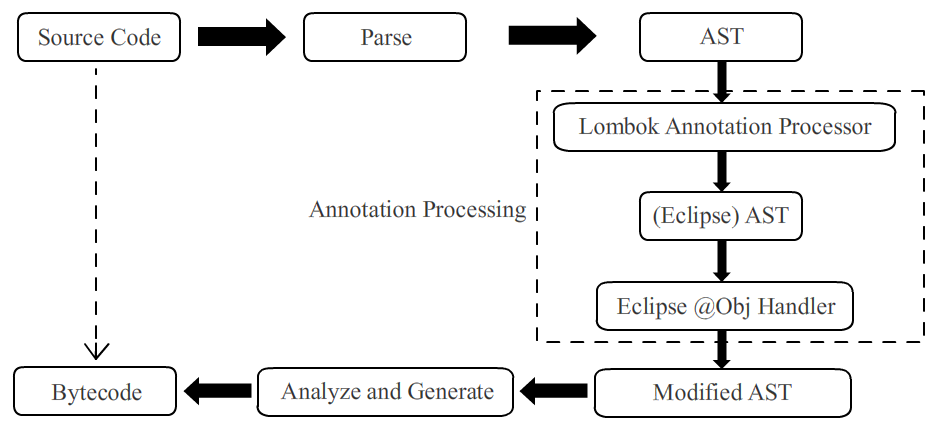
\includegraphics[width=5in]{pdfs/lombok.png}
\caption{The flow chart of Lombok annotation processing. [Ref: http://notatube.blogspot.hk/2010/12/project-lombok-creating-custom.html]
\marco{I'm not sure this helps: It is trying to show the "eclipse" path, that is the one we implemented,
but there is also the "javac" path, and here we call the graph "Lombok annotation processing".
May be this should be "obj" processing?
}}
\end{figure*}

Our implementation is based on an extension of Lombok. The Lombok
project~\cite{lombok} is a Java library that aims at removing (or
reducing) Java boilerplate code via
annotations. There are a number of annotations provided by the
original Lombok, including \Q:@Getter:, \Q:@Setter:,
\Q:@ToString: for generating getters, setters and \QM{toString}
methods, respectively.  Furthermore, Lombok provides a number of
interfaces for users to create custom transformations, as extensions
to the original framework.
A transformation is based on a handler, which acts on the AST for the
annotated node and returns a modified AST for analysis and
generation afterwards. Such a handler can either be a Javac handler or
an Eclipse handler.

The annotation we created is \mixin. Figure~\ref{fig:lombok}\haoyuan{Wrong ref?} illustrates the
flow of \mixin annotation processing in Lombok. In Eclipse, with an interface annotated by
\mixin, the automatic annotation processing is performed transparently and the information of
the interface from compilation is captured in the ``Outline'' window. This includes
all the methods inside the interface as well as the generated ones.  The custom
transformation is easy and convenient to use.  For example, this means that the
IDE functionality for content assist and autocomplete will work for the newly generated
methods. The biggest reasons to use Lombok rather than using a conventional Java
 annotation processor are:
\begin{itemize}
%this seems like a commercial spot
%\item Lombok is byte-code based instead of source-code based, which makes client
%  code concise and easy to maintain. Such code generation is performed at
%  compile time to modify bytecode.
\item Lombok modifies the generation process of the class files, by directly modifying the AST.
Neither the source code is modified nor new Java files are generated.
\item Moreover, and probably more importantly, Lombok is capable of generating
  code \emph{inside} a class/interface, which conventional
  Java annotation processors do not support.
\end{itemize}

\noindent
Lombok offers several advantages over conventional code preprocessors/macros,
and our disciplined \mixin annotation offer some more advantages with respect to arbitrary Lombok-based
AST rewriting.
\begin{itemize}
\item \textbf{Lack of modularity.}
While general preprocessing can act across module boundaries, Lombok acts modularly on each class, and it makes
sense to apply the transformation to one class/interface at a time, and only to annotated classes/interfaces.
This allows library code to be reused without the need of being
reprocessed and recompiled.

\item \textbf{Syntax and type errors.}
Some preprocessors (like the C one) can produce syntactically invalid code.
Lombok ensures only syntactically valid code is produced; however, type errors can appear.
In our annotation, we prove that we do not introduce new errors in clients (see Section~\ref{subsec:guarantees} and Section~\ref{subsec:results} for details).

\item \textbf{Obfuscated source code.}
Preprocessors bring great power, which can easily be misused producing
code particularly hard to understand. Thus code quality and maintainability are reduced.
Lombok requires to start from Java syntax, and can reinterpret it.
This is already better, since the syntax is preserved, but the reinterpretation could be surprising for
badly designed Lombok-based rewritings.
However, the``Outline'' window of Eclipse or other IDEs (and thus their auto-completion facilities)
will show the result of the rewriting, helping the programmer to use the reinterpreted semantic.

Our annotation reinterpret the syntax for the sole goal of enhance/complete code:
we satisfy the behaviour of abstract methods, we add methods and we refine return types.
We consider this to be quite easy to follow, since it is similar to what happens in normal inheritance.

\marco{The section No reuse of the type system
is controversial.
We do need to repeat the type checking, plus we aim to make untypable stuff well typed
(for example anyone using the of method would not be well typed before).}
%\item \textbf{No reuse of the type system.}
%As we mentioned above, badly designed rewritings can arise from the great power of Lombok. A simple piece of source code
%\begin{lstlisting}
%interface M { int m(); }
%\end{lstlisting}
%can be reinterpreted as
%\begin{lstlisting}
%interface M { void m(String s); }
%\end{lstlisting}
%in which case the type of method \Q@m@ is changed. Our \mixin annotation does not introduce this kind of rewritings,
%and hence the type system is reused. Moreover, Lombok can also modify unbounded types, which is easy to understand,
%for instance, the following code
%\begin{lstlisting}
%interface M { T m(); } // T is unbounded
%\end{lstlisting}
%is transformed into
%\begin{lstlisting}
%interface M { int m(); } // No error message
%\end{lstlisting}
%in which case the user will see the unbounded type in source code, but without error message from the compilation, since
%Lombok has modified the return type of \Q@m@. However, our \mixin annotation can still keep such errors and warnings.


%\item \textbf{Lack of reuse.}  %not sure here... I think most preprocessors support decent reuse, even the C one
%Reusability is yet another concern in using preprocessors.
% In Lombok, implementations of features are
%encapsulated in various annotation handlers,
% in which case some behaviours are allowed to reuse the code by invoking methods
%in other handlers, where tedious replicated code is avoided.
\end{itemize}

\paragraph{Limitations}
Our prototype implementation using Lombok has certain limitations:
\begin{itemize}
\item The prototype does not support separate compilation yet. Currently all
  related interfaces have to appear in a single Java file. Therefore, changes to
  a single interface would require re-compiling the whole file. This compilation
  limitation is not caused by our algorithm. It is a Lombok implementation related
  issue: in Lombok it is hard to capture a type declaration from its reference,
  even harder when the type declaration is in other files (we have not found a
  way to do this yet).
\item At this stage our implementation only realizes the Eclipse handler and our
  experiments are all conducted in Eclipse. The implementation for
  \texttt{javac} is missing.
\item The current implementation does not take type-parameters into
  consideration, thus it does not support generics yet.
\end{itemize}

\paragraph{Comparison with other Lombok annotations}
The Lombok project provides a set of predefined annotations, including constructor
generators similar as ours (e.g., \Q:@NoArgsConstructor:,
\Q:@RequiredArgsConstructor: and \Q:@AllArgsConstructor:). They
generate various kinds of constructors for \emph{classes}, with or without
constructor arguments. This set of annotations is of great use, especially when
used together with other features provided in Lombok (e.g.,
\Q:@Data:). Moreover, the implementation of these annotations in Lombok
gives us hints on how to implement \mixin. However, none of these annotations
can model what we are doing with \mixin - generating constructor-methods
(\textbf{of}) for \emph{interfaces}. Apart from constructors, \mixin also
provides other convenient features (including generating fluent setters, type
refinement, etc), which the base Lombok project does not provide.
Finally, while \mixin is formalized, none of Lombok's annotations have been
studied in a formal way.

\paragraph{Lombok does language tuning}
We consider Lombok to be the most developed example of language
tuning.  While the authors of Lombok do not introduce a specific term
for what they are doing, their slogan \emph{``Spice up your java''}
seems to be in line with the philosophy of language tuning. Some
other examples of language tuning in Lombok include the \Q@val@ type,
similar to \Q@auto@ in C\# or C++04.  Another library doing language
tuning is CoFoJa~\cite{cofoja}, where annotations are used to insert
pre-post conditions in generated bytecode.


